\documentclass[12pt,oneside,a4paper]{article} % for sharing
\usepackage{apacite}
\usepackage{appendix}
\usepackage{amsmath}
\usepackage{amsthm}
\usepackage{multirow}
\usepackage{amssymb} % for approx greater than
\usepackage{caption}
\usepackage{placeins} % for \FloatBarrier
\usepackage{graphicx}
\usepackage{subcaption}
\usepackage{longtable}
\usepackage{setspace}
\usepackage{booktabs}
\usepackage{tabularx}
\usepackage{xcolor,colortbl}
\usepackage{chngpage}
\usepackage{natbib}
\bibpunct{(}{)}{,}{a}{}{;} 
\usepackage{url}
\usepackage{nth}
\usepackage{authblk}
\usepackage[most]{tcolorbox}
\usepackage[normalem]{ulem}
\usepackage{amsfonts}
% columns for longtable
\newcolumntype{C}[1]{>{\centering\let\newline\\\arraybackslash\hspace{0pt}}m{#1}}
\newcolumntype{L}[1]{>{\raggedright\let\newline\\\arraybackslash\hspace{0pt}}m{#1}}
\usepackage{arydshln} % Dashed lines in matrices

\usepackage[margin=1in]{geometry}
%\doublespacing % for review

% line numbers to make review easier
%\usepackage{lineno}
%\linenumbers

%\usepackage{soul}% for \st{}

%%%%%%%%%%%%%%%%%%%%%%%%%%%%%%%%%%%%%%%%%%%%%%%%%%%%%%%%%%%%%%%%%%%%%%%%%%%%%%
% for section 4 math environments
\theoremstyle{definition}
\newtheorem{definition}{Definition}[section]
\newtheorem{theorem}{Theorem}[section]
\newtheorem{proposition}{Proposition}[section]
\newtheorem{corollary}{Corollary}[proposition]
\newtheorem{remark}{Remark}[section]

%%%%%%%%%%%%%%%%%%%%%%%%%%%%%%%%%%%%%%%%%%%%%%%%%%%%%%%%%%%%%%%%%%%%%%%%%%%%%%

\newcommand\ackn[1]{%
  \begingroup
  \renewcommand\thefootnote{}\footnote{#1}%
  \addtocounter{footnote}{-1}%
  \endgroup
}

% Affiliations in small font size
\renewcommand\Affilfont{\small}

\defcitealias{HMD}{HMD 2016}

% junk for longtable caption
\AtBeginEnvironment{longtable}{\linespread{1}\selectfont}
\setlength{\LTcapwidth}{\linewidth}

% sort van Raalte properly
% #1: sorting key, #2: prefix for citation, #3: prefix for bibliography
\DeclareRobustCommand{\VAN}[3]{#2} % set up for citation

%%%%%%%%%%%%%%%%%%%%%%%%%%%%%%%
\begin{document}

\title{A decomposition of longevity inquality by deprivation quantiles}
%\author{author(s) redacted}
\author[1]{Rosie Seaman\thanks{seaman@demogr.mpg.de}}
\author[2]{Hal Caswell}
\author[1]{Tim Riffe}

\affil[1]{Max Planck Institute for Demographic Research, Rostock, Germany}
\affil[2]{University of Amsterdam}

\maketitle

\begin{abstract}
Within-variance is way bigger than between variance we suppose. Let's see. And
also see how it changes over age and time.
\end{abstract}

\section{Data and methods}

\subsection{Variance decomosition}

We have a set of lifetables for subareas of Scotland
that can be assigned to deprivation quantiles. The index $k$ refers to
subpopulations. Given $p_x = 1- q_x$ for a subpopualtion, calculate:
\begin{equation}
\mathbf{U}_k = 
\begin{bmatrix}
    0     & \hdots  & \hdots &  \hdots  & 0 \\
    p_{1} &   &    &    &  \vdots \\
    0 & \ddots &   &   & \vdots \\
    \vdots & & \ddots & & 0\\
   0 &  \hdots & 0 & p_{\omega-1}  & p_{\omega}
\end{bmatrix}
\end{equation}
Then calculate the conditional remaining survivorship as
\begin{equation}
\mathbf{N}_k = (\mathbf{I} - \mathbf{U}_k )^{-1} \quad .
\end{equation}
$\mathbf{N}_k$ ends up being 0s in the upper triangle, and conditional remaining
survivorship in columns descending from the subdiagonal. The first moment is the
same as remaining life expectancy, and can be calculated as:
\begin{equation}
\eta^{(k)}_1 = (1^T \mathbf{N}_k)^T
\end{equation}
The second moment is defined as:
\begin{equation}
\eta^{(k)}_2 = \left[ 1^T \mathbf{N}_k (2\mathbf{N}_k - \mathbf{I})\right]^T
\end{equation}
These can be used together to calculate the variance of remaining lifespan:
\begin{equation}
\label{eq:var}
V(\eta^{(k)}) = \eta^{(k)}_2 - \left[\eta^{(k)}_1 \circ \eta^{(k)}_1 \right]
\end{equation}
Thus far everything has been denoted with respect to the $k^{th}$ subpopulation.
These may aggregate to a total lifetable according to some mixing distribution,
$\pi$.
The most natural mixture is to to give age-specific weights according to
observed relative population counts in each subpopulation, $\pi(a,k)$. Other
mixtures may be based on an age-pattern to $\pi$ based on the stationary
population produced by each subpopulation's lifetable. By this method, lower
mortality lifetables result in greater relative weight in older ages. In this
case, weight is assigned only to the lifetable radix. Good choice might be
assigning weight relative to the total population size of each area, or simply
giving uniform weights. Since in our case subpopulations are aggregated into
deprivation quantiles, they end up being of approximately equal size and the
uniform radix mixing distribution is not very bad. 

Given $\pi(a,k)$ we can decompose the variance of the total
aggregation of subpopulations due to \eqref{eq:var} into variance due to
stochasticity within subpopulations and variance due to differences between
populations in the lifespan distribution. These two variance components sum to
\eqref{eq:var} when the same $\pi(a,k)$ is used to blend lifetables for
\eqref{eq:var} and in the following equations:
\begin{align}
V_{within} &= \mathbb{E}_\pi \left( V(\eta_1^{(k)})\right)\\
 &= \sum_{k=1}^N \pi_k V(\eta_1^{(k)})
\intertext{and}
V_{between} &= V_\pi \left( V(\eta_1^{(k)})\right)\\
 &= \sum_{k=1}^N \pi_k \circ \eta_1^{(k)} \circ \eta_1^{(k)} -
 \left[ \sum_{k=1}^N \pi_k \circ \eta_1^{(k)} \right] \circ \left[ \sum_{k=1}^N \pi_k
 \circ \eta_1^{(k)} \right]
\end{align}



\section{Results}

First some descriptives.


Now some graphs:

\begin{figure*}[t!]
    \centering
      \caption{Standard deviation of remaining lifespan by age, census years
      1981 until 2011.}
    \begin{subfigure}[t]{0.5\textwidth}
        \centering
        \caption{Females}
        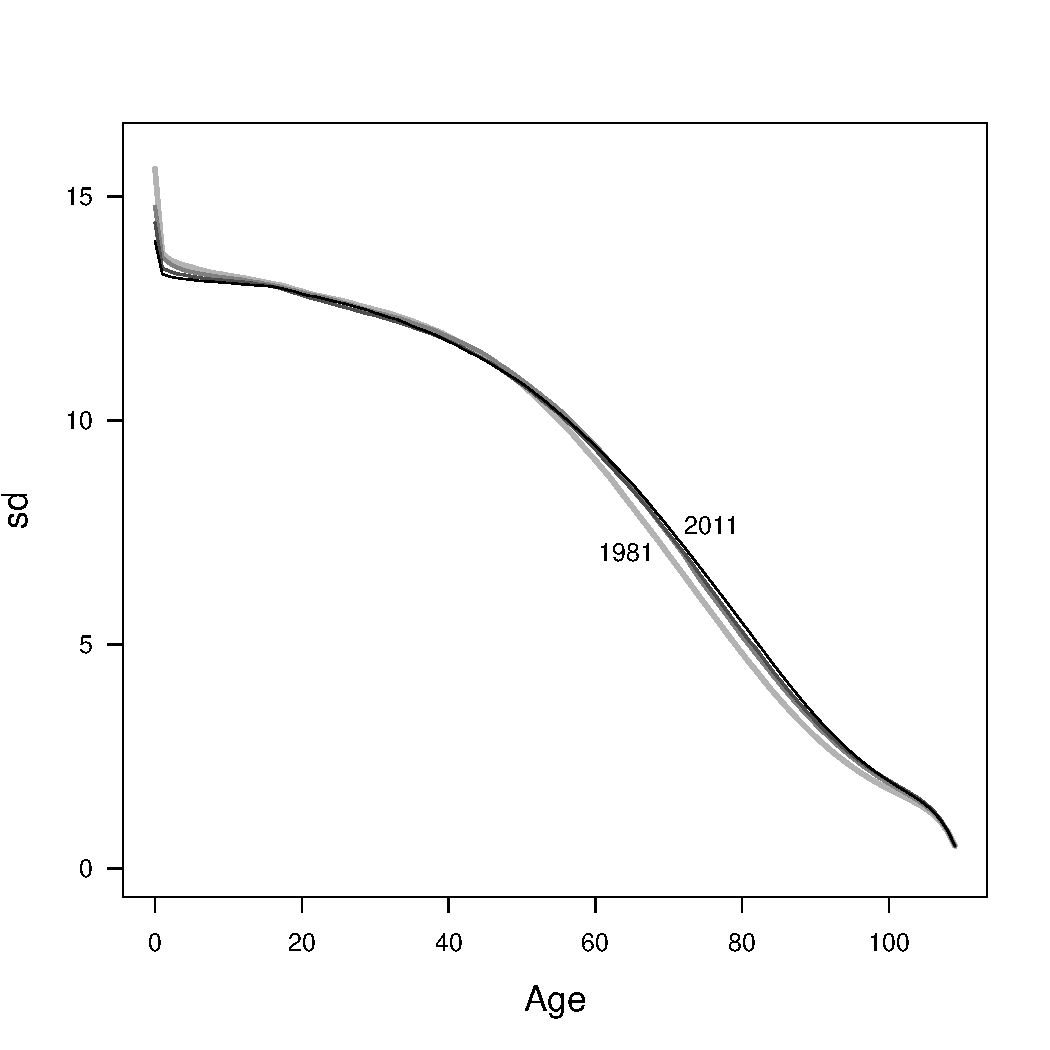
\includegraphics[width=\textwidth]{Figures/TotalsdFemales.pdf}
    \end{subfigure}%
    ~ 
    \begin{subfigure}[t]{0.5\textwidth}
        \centering
        \caption{Males}
        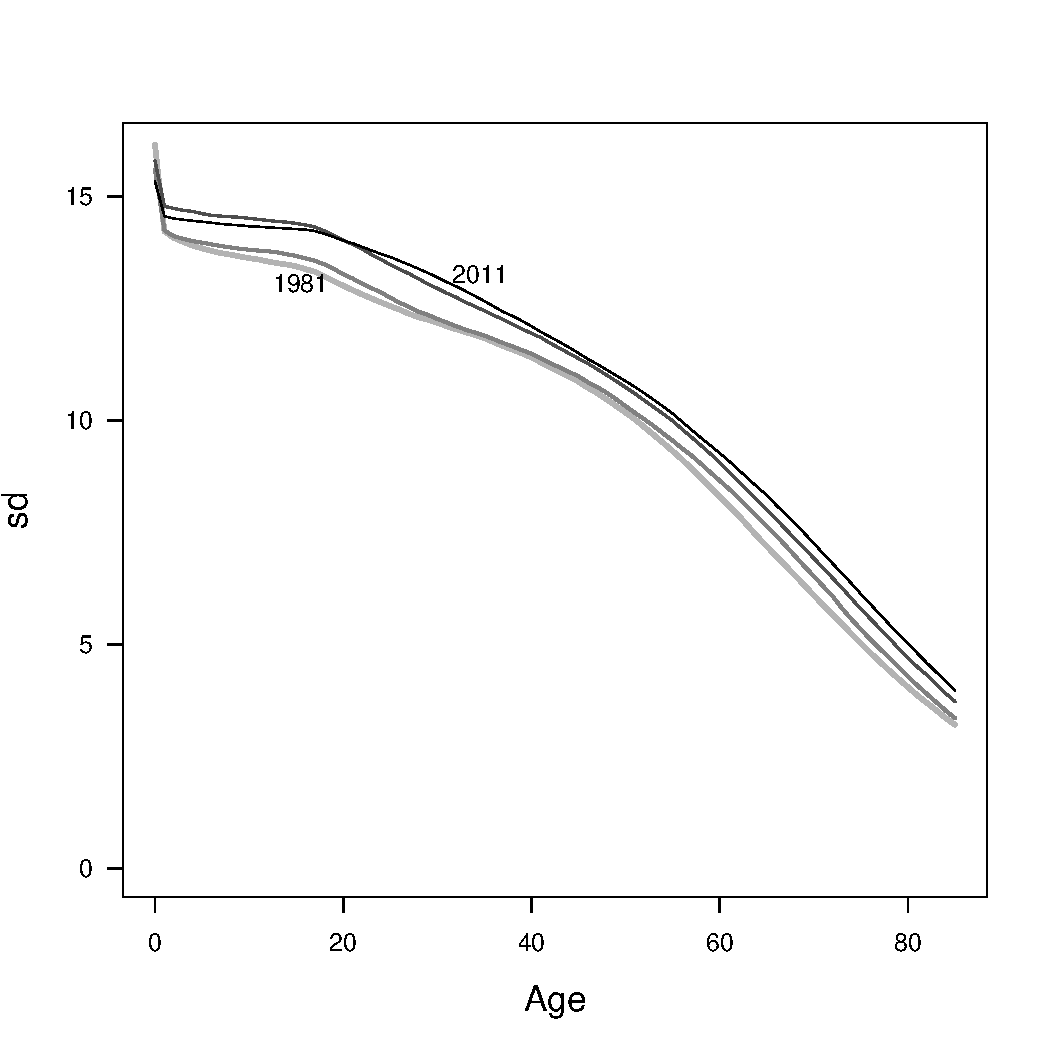
\includegraphics[width=\textwidth]{Figures/TotalsdMales.pdf}
    \end{subfigure}
\end{figure*}


\begin{figure*}[t!]
    \centering
      \caption{Proportion of variance due to differences between deprivation
      quintiles by age, census years 1981 until 2011.}
    \begin{subfigure}[t]{0.5\textwidth}
        \centering
        \caption{Females}
        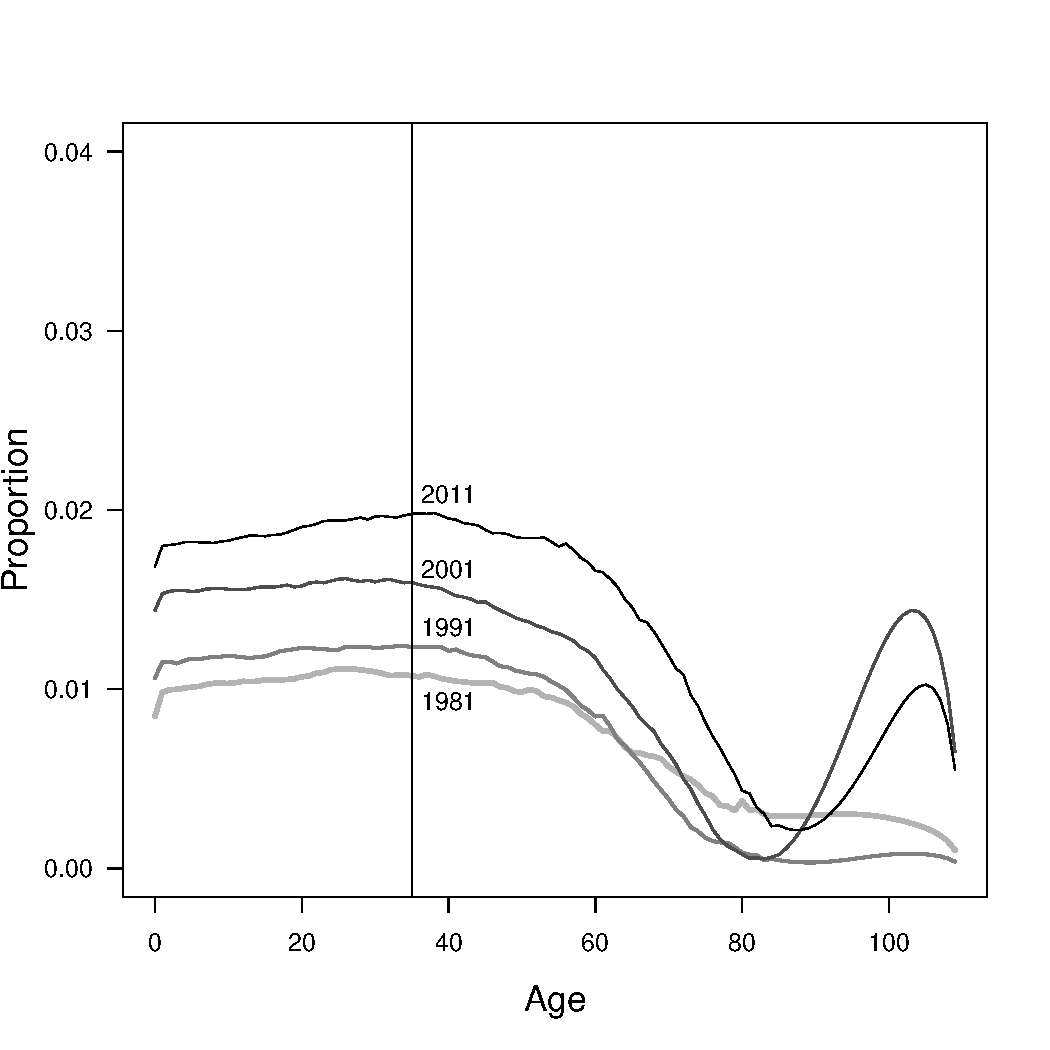
\includegraphics[width=\textwidth]{Figures/BetweenPropFemales.pdf}
    \end{subfigure}%
    ~ 
    \begin{subfigure}[t]{0.5\textwidth}
        \centering
        \caption{Males}
        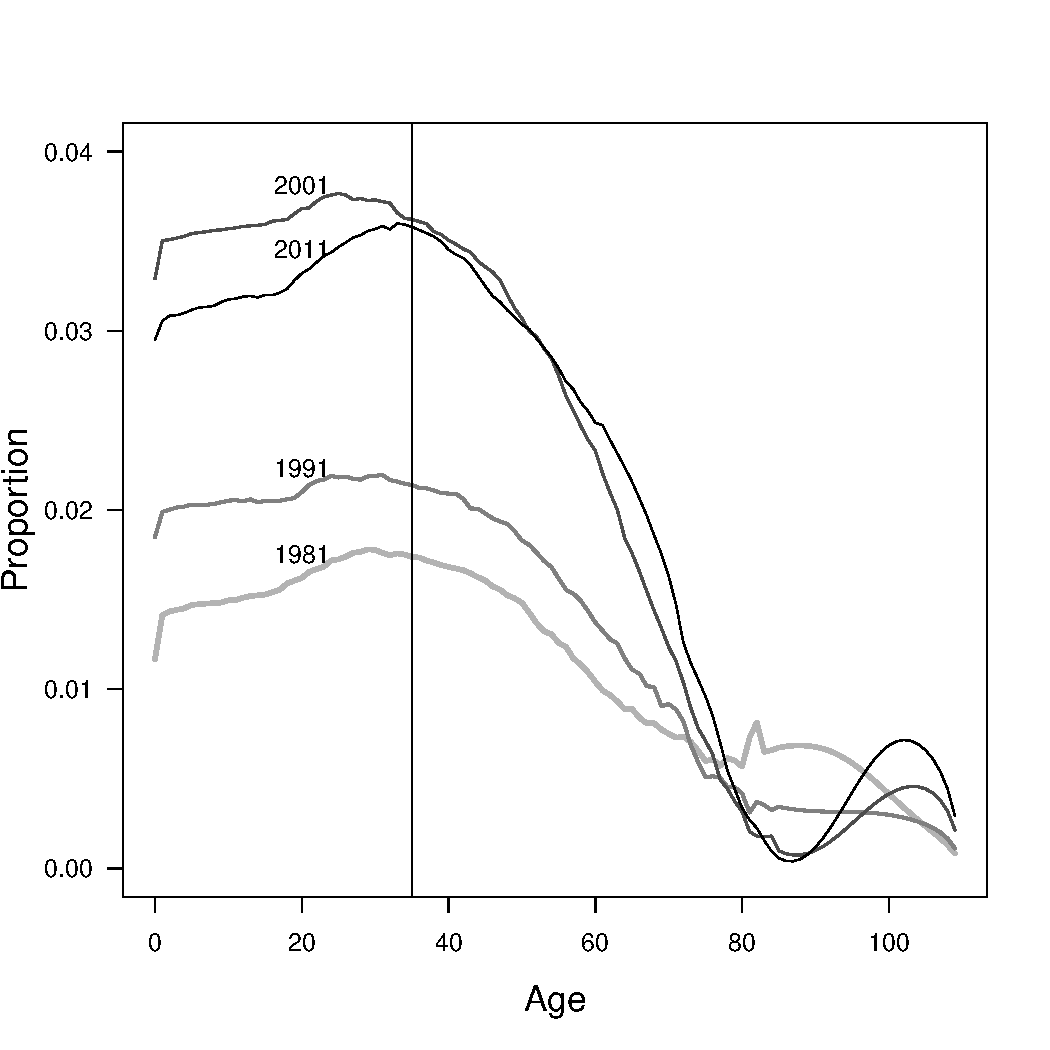
\includegraphics[width=\textwidth]{Figures/BetweenPropMales.pdf}
    \end{subfigure}
\end{figure*}


\end{document}
